\documentclass[11pt, oneside]{article}   	% use "amsart" instead of "article" for AMSLaTeX format
\usepackage{geometry}                		% See geometry.pdf to learn the layout options. There are lots.
\geometry{letterpaper}                   		% ... or a4paper or a5paper or ... 
%\geometry{landscape}                		% Activate for rotated page geometry
%\usepackage[parfill]{parskip}    		% Activate to begin paragraphs with an empty line rather than an indent
\usepackage{graphicx}				% Use pdf, png, jpg, or eps§ with pdflatex; use eps in DVI mode
								% TeX will automatically convert eps --> pdf in pdflatex		
\usepackage{amssymb}
\usepackage{amsmath}
\usepackage{float}
%SetFonts

\usepackage[utf8]{inputenc}
\newcommand{\Var}{\operatorname{Var}}
% Default fixed font does not support bold face
\DeclareFixedFont{\ttb}{T1}{txtt}{bx}{n}{12} % for bold
\DeclareFixedFont{\ttm}{T1}{txtt}{m}{n}{12}  % for normal

% Custom colors
\usepackage{color}
\definecolor{deepblue}{rgb}{0,0,0.5}
\definecolor{deepred}{rgb}{0.6,0,0}
\definecolor{deepgreen}{rgb}{0,0.5,0}

\usepackage{listings}

% Python style for highlighting
\newcommand\pythonstyle{\lstset{
language=Python,
basicstyle=\ttm,
otherkeywords={self},             % Add keywords here
keywordstyle=\ttb\color{deepblue},
emph={MyClass,__init__},          % Custom highlighting
emphstyle=\ttb\color{deepred},    % Custom highlighting style
stringstyle=\color{deepgreen},
frame=tb,                         % Any extra options here
showstringspaces=false            % 
}}


% Python environment
\lstnewenvironment{python}[1][]
{
\pythonstyle
\lstset{#1}
}
{}

% Python for external files
\newcommand\pythonexternal[2][]{{
\pythonstyle
\lstinputlisting[#1]{#2}}}

% Python for inline
\newcommand\pythoninline[1]{{\pythonstyle\lstinline!#1!}}

\title{Mixed signal processing and machine learning methods for bearings fault detection: Application in predictive meantenance (Project outline)}
\author{Yapi Donatien Achou}
%\date{}							% Activate to display a given date or no date

\begin{document}


\maketitle
\tableofcontents
\newpage
%\begin{figure}[H] %  figure placement: here, top, bottom, or page
%   \centering
%   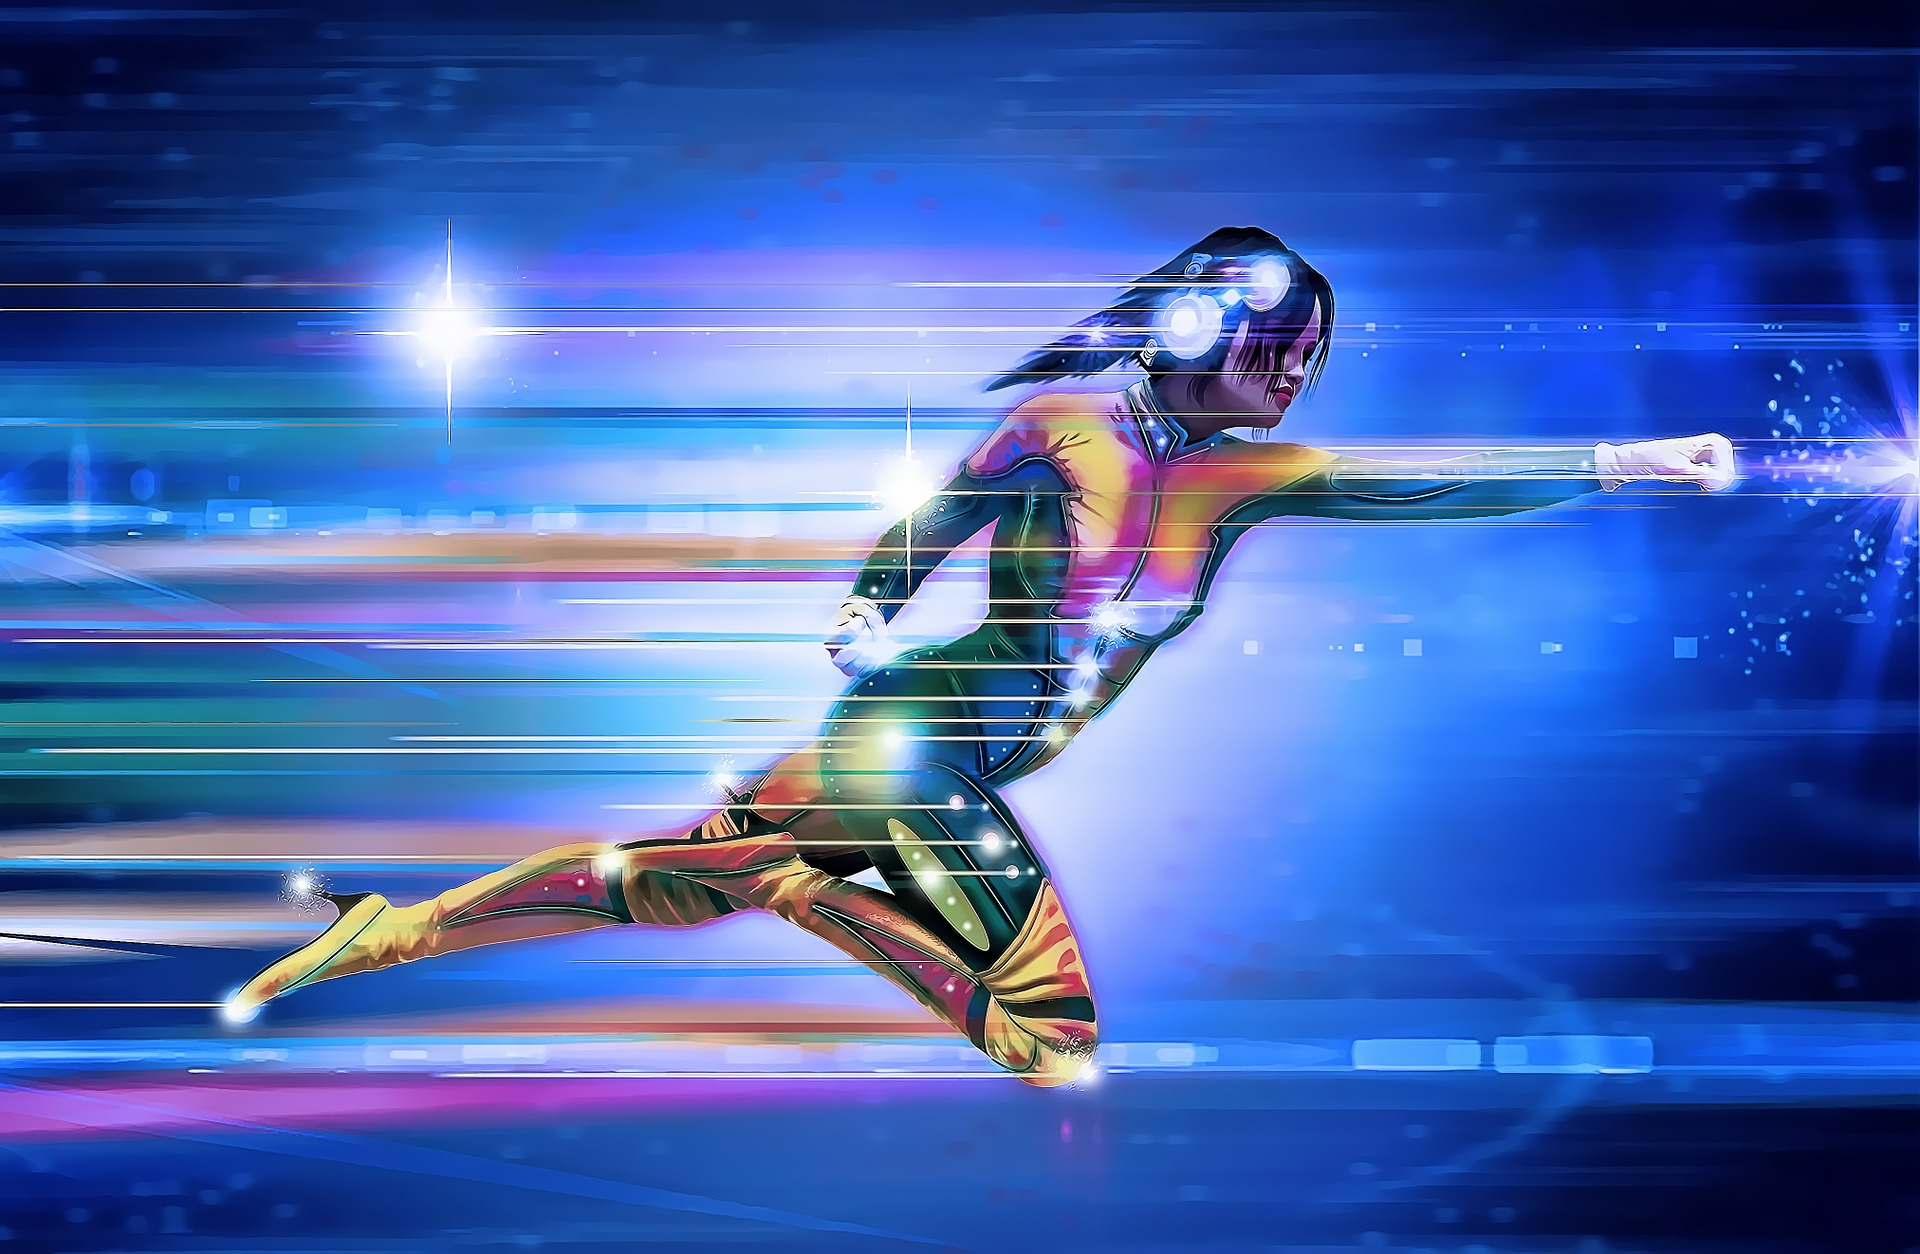
\includegraphics[width=5in]{front4} 
%   \caption{}
%   \label{fig:example}
%\end{figure}
\section{Introduction}
Predictive maintenance can be defined as a maintenance philosophy with a set of methods used to predict and prevent machine failure in order to avoid unexpected downtime. This maintenance philosophy when correctly implemented, increases machine life time, and reduces maintenance cost [referecne].
\begin{flushleft}
In rotating machines, more than 40 $\%$ of machine malfunction can be attributed to bearing defect [references]. 
\end{flushleft}
\begin{figure}[H] %  figure placement: here, top, bottom, or page
   \centering
   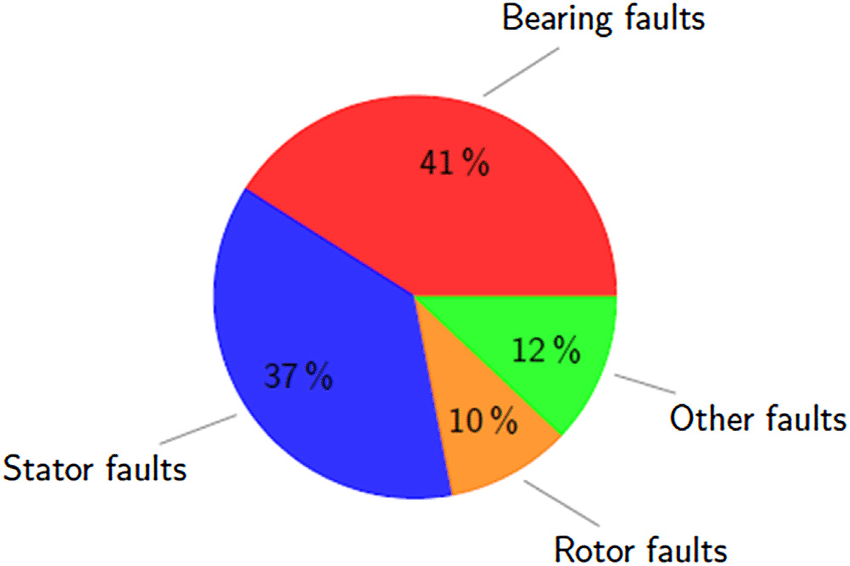
\includegraphics[width=5in]{pie.png} 
   \caption{Defect statistic, taken from [reference]}
   \label{fig:pie}
\end{figure}
In this project we present a mixed methodology to detect and predict bearing defects. The methodology consists of using signal processing for feature generation and data labelling,  and machine learning for defects classification and failure prediction. For a given input dataset, the dataset is decomposed into it subcomponents or basis components. The basis components also called features are then used as input of a supervised learning algorithm for defect classification and failure prediction.
\begin{flushleft}
The signal processing methods used are Fourier transform, wavelet transform and Hilbert Huang transform. We focus on ensemble learning and feed forward neural network for classification. Furthermore we show that the back-propagation process in the feed forward neural network can be modelled by an ordinary differential equation, whose solution represents the path of the hidden and output layer weights.
\end{flushleft}


\begin{flushleft}
The outline of the project is as followed: In section (chapter) one we give an overview of the signal processing methods. In section (chapter) two we present the machine learning methodology and show that the back-propagation in the feedforward neural network can be modelled as a differential equation.
In section (chapter) 3 we present a case study where we apply the methodology defined in section one and two. In section four we present the conclusion of this work.
\end{flushleft}

%%%%%%%%%%%%%%%%%%%%%%%%%%%%%%%%%%%%%%%%%%%%%%%%%%%%%%%%%%%%%%%%%%%%%%%%%%%%%%%%%%%%
%%%%%%%%%%%%%%%%%%%%%%%%%%%%%%%%%%%%%%%%%%%%%%%%%%%%%%%%%%%%%%%%%%%%%%%%%%%%%%%%%%%%
%%%%%%%%%%%%%%%%%%%%%%%%%%%%%%%%%%%%%%%%%%%%%%%%%%%%%%%%%%%%%%%%%%%%%%%%%%%%%%%%%%%%

\section{Preview work}
%%%%%%%%%%%%%%%%%%%%%%%%%%%%%%%%%%%%%%%%%%%%%%%%%%%%%%%%%%%%%%%%%%%%%%%%%%%%%%%%%%%%
%%%%%%%%%%%%%%%%%%%%%%%%%%%%%%%%%%%%%%%%%%%%%%%%%%%%%%%%%%%%%%%%%%%%%%%%%%%%%%%%%%%%
%%%%%%%%%%%%%%%%%%%%%%%%%%%%%%%%%%%%%%%%%%%%%%%%%%%%%%%%%%%%%%%%%%%%%%%%%%%%%%%%%%%%

\section{Signal processing methods}
\subsection{Overview}
We present three signal processing methods for data decomposition or feature generation. The three methods can be described as follow: Given a dataset  approximated by a map
\begin{equation}
f: \mathbb{R} \rightarrow \mathbb{R}
\end{equation}
find a space $V$ spanned by a basis $\{ \varphi_{j} \}_{j=0}^{n}$ such that 
\begin{equation}
f(x) = \sum_{j=0}^{j=n}\alpha_{j}\varphi_{j}.
\end{equation}
In the context of this work, the basis functions $\{ \varphi_{j} \}_{j=0}^{n}$ are the features derived from the original dataset.
\subsection{Fourier transform}
\subsubsection{Theory}
\subsubsection{Application}



%%%%%%%%%%%%%%%%%%%%%%%%%%%%%%%%%%%%%%%%%%%%%%%%%%%%%%%%%%%%%%%%%%%%%%%%%%%%%%%%%%%
%%%%%%%%%%%%%%%%%%%%%%%%%%%%%%%%%%%%%%%%%%%%%%%%%%%%%%%%%%%%%%%%%%%%%%%%%%%%%%%%%%%
\subsection{Wavelet transform}
\subsubsection{Theory}
\subsubsection{Application}



%%%%%%%%%%%%%%%%%%%%%%%%%%%%%%%%%%%%%%%%%%%%%%%%%%%%%%%%%%%%%%%%%%%%%%%%%%%%%%%%%%%
%%%%%%%%%%%%%%%%%%%%%%%%%%%%%%%%%%%%%%%%%%%%%%%%%%%%%%%%%%%%%%%%%%%%%%%%%%%%%%%%%%%
\subsection{Hilbert Huang transform}
\subsubsection{Theory}
The Hilbert-Huang transform is a data decomposition methods that consists of decomposing data in an adaptive fashion. Adaptivity means that rather than imposing an a priory basis such as trigonometric functions, a posteriori basis functions are derived from the data itself \cite{norden2008}. In doing so, the method deals better with nonlinearity and non stationarity which are inherently present in real world data.

\begin{flushleft}
This method gives an alternative approach of time-frequency-energy paradigm by using Hilbert spectral analysis and the so call empirical mode decomposition (EMD) to express the nonlinearity and the non stationary in data 
with instantaneous frequency and instantaneous amplitude \cite{norden2008}.
\end{flushleft}
\begin{flushleft}
The empirical mode decomposition (EMD) originated from the quest of functions that can be expressed by a time-frequency-amplitude expression, such that the frequency is physically meaningful.
Consider a time series $x(t)$. Its Hilbert transform H(t) is given by 

\begin{equation}
H(t) = \frac{1}{\pi}P\int_{_\infty}^{\infty}\frac{x(\tau)}{t-\tau}\mathrm{d}\tau,
\end{equation}
where $P$ is the Cauchy principal value. The corresponding time-frequency-amplitude function of $x(t)$ is the analytical function
\begin{equation}
z(t) = x(t) + iy(t) = a(t)e^{i\theta(t)},
\end{equation}
where the instantaneous amplitude $a(t)$ and phase $\theta(t)$ can be computed by 
\begin{equation}\label{eq:amp}
a(t) = \sqrt{x(t)^{2}+ y(t)^{2}}
\end{equation}
\begin{equation}
\theta(t) = \tan^{-1}\left(\frac{y(t)}{x(t)}\right).
\end{equation}
Furthermore, the instantaneous frequency $w(t)$ can be derived from the phase $\theta(t)$ as
\begin{equation}\label{eq:freq}
w(t) = \frac{d\theta}{dt}.
\end{equation}
By setting 
\begin{equation}
f(t) = \frac{y(t)}{x(t)}, \nonumber
\end{equation}
the expression of the instantaneous  amplitude $w(t)$ in (\ref{eq:freq}) can be expanded as
\begin{equation}
w(t) = \frac{f^{\prime}(t)}{1+f(t)^{2}} = \frac{y^{\prime}(t)x(t)-y(t)x^{\prime}(t)}{x(t)(x(t)+y(t)^{2})}.
\end{equation}
The instantaneous frequency $w(t)$ using the Hilbert transform is not always physically meaning. For example for an arbitrarily function, the instantaneous physical frequency values should be positive. However this is not always the case. 

\begin{flushleft} 
For example if 
\begin{equation}
f(x) = \cos(ct) +d 
\end{equation}
where $c$ and $d$ are constants, the instantaneous frequency is given by
\begin{equation}
w(t) = \frac{-c\sin(ct)}{1+(\cos(ct) +d)^{2} }
\end{equation}
\begin{figure}[H] %  figure placement: here, top, bottom, or page
   \centering
   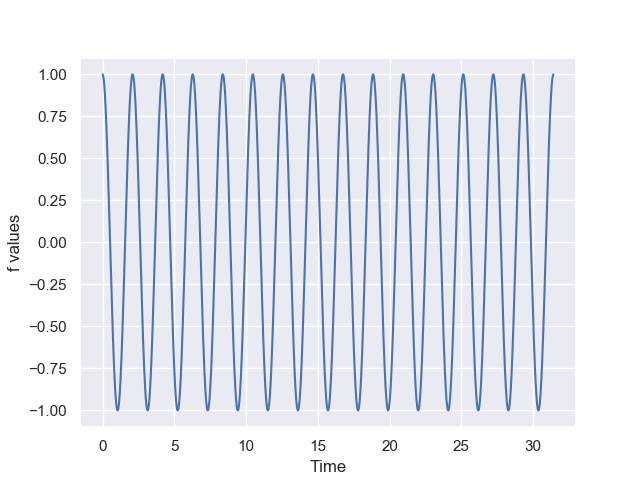
\includegraphics[width=2.5in]{f} 
     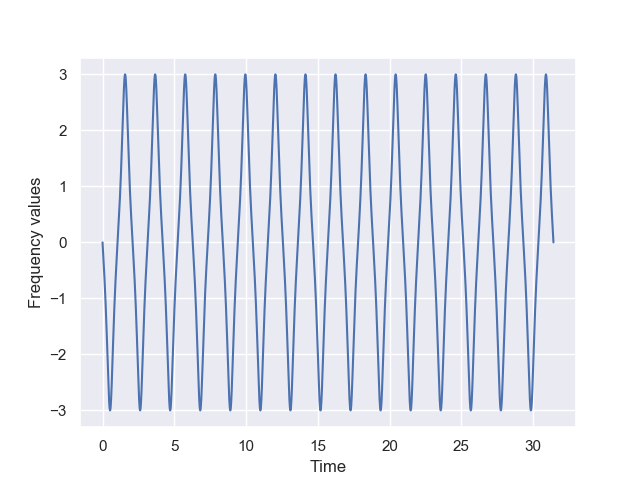
\includegraphics[width=2.5in]{frequency} 
   \caption{function f and its corresponding frequency}
   \label{fig:freq}
\end{figure}
From Figure \ref{fig:freq}, we see that the instantaneous frequency takes negative values, which is not physically meaning full. 
\end{flushleft}

\begin{flushleft}
To circumvent this, the Hilbert-Huang transform offers a methodology to obtain from an arbitrarily function or time series $x(t)$ a set of finite subcomponents whose instantaneous frequency are physically meaningful. This methodology let to the empirical mode decomposition.
\end{flushleft}



%Once the instantaneous frequency and amplitude are defined, we can define the Hilbert-Huang spectrum H(w,t), \cite{hui2007} as 
%\begin{equation}\label{eq:hs}
%H(w,t) = Re\sum_{i=1}^{n}a_{i}(t)\exp\left(\int w_{i}(t)\mathrm{d}t\right),
%\end{equation}
%and compute the marginal spectrum 
%\begin{equation}
%h(w) = \int_{0}^{T}H(w,t)\mathrm{d}t.
%\end{equation}
%While the Hilbert spectrum is the energy contribution of each instantaneous frequency, the marginal spectrum is the total energy contribution of all instantaneous frequency
%\cite{norden2008, hui2007}. 
\end{flushleft}

\begin{flushleft}
 The necessary condition for obtaining a physical frequency is that $x(t)$ satisfies the approximate local envelope symmetry condition \cite{norden1998}. 



This condition 
is expressed in the empirical mode decomposition (EMD) such that an arbitrarily time series $x(t)$ can be decomposed by a sifting process into intrinsic mode function $c_{i}$
\begin{equation}
x(t) = \sum_{i=1}^{n}c_{i} + r_{n}
\end{equation}
where the $c_{i}$ satisfies the approximate local envelope symmetry condition
\begin{equation}
SD_{k} = \frac{\sum_{t=0}^{T}}{\sum_{t=0}^{T}} < \epsilon
\end{equation}
where $\epsilon$ is a small predefined real number.
\end{flushleft}

\subsubsection{Application for bearings fault detection}
we consider a vibration signal with sample frequency of 20000Hz rotating speed of 2000 RPM
\begin{figure}[H] %  figure placement: here, top, bottom, or page
   \centering
   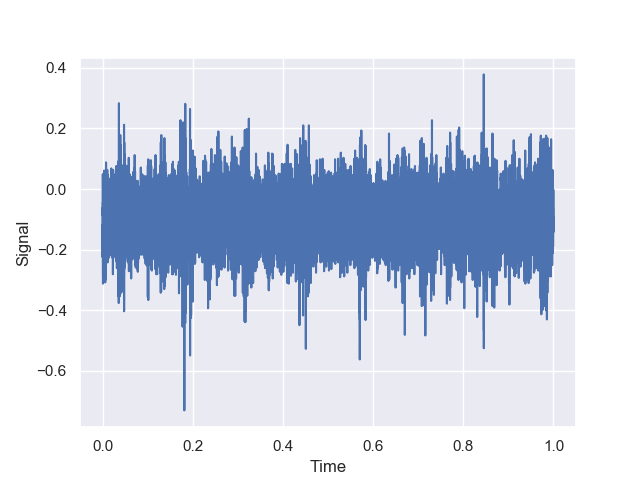
\includegraphics[width=4in]{signal} 
   \caption{Vibration signal of 1 second snapshot}
   \label{fig:signal}
\end{figure}
\begin{flushleft}
After applying the empirical mode decomposition on the vibration data from figure \ref{fig:signal} we get sixteen  intrinsic mode functions
\begin{figure}[H] %  figure placement: here, top, bottom, or page
   \centering
   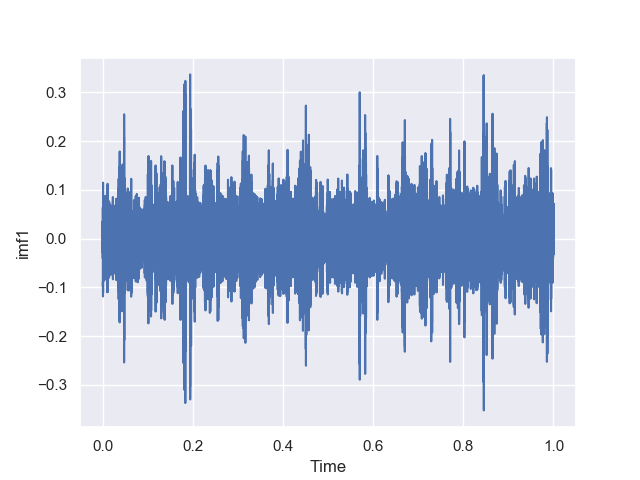
\includegraphics[width=2.5in]{imf/imf1.png} 
     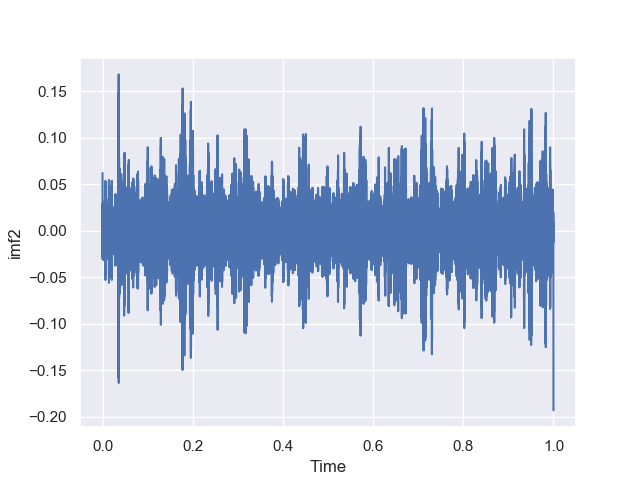
\includegraphics[width=2.5in]{imf/imf2.png} 
   \caption{1th and 2nd intrinsic mode function (imf)}
   \label{fig:imf11}
\end{figure}

\begin{figure}[H] %  figure placement: here, top, bottom, or page
   \centering
   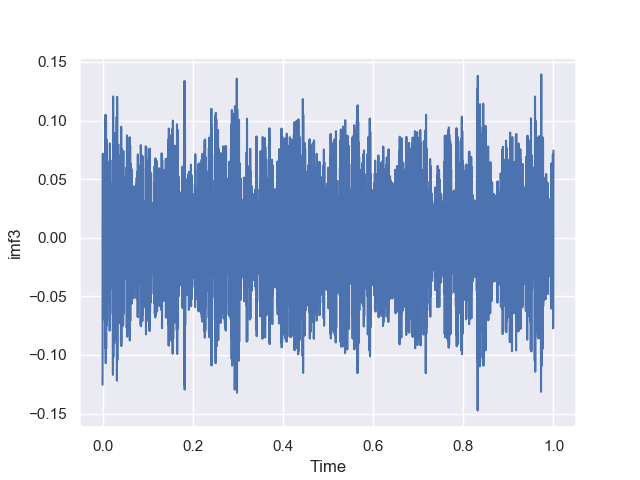
\includegraphics[width=2in]{imf/imf3.png} 
     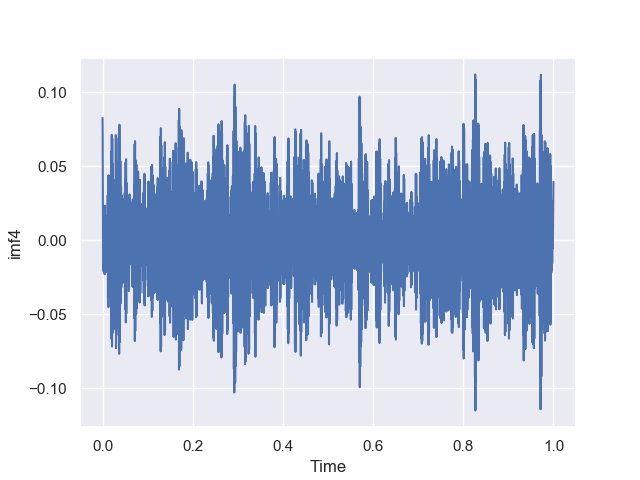
\includegraphics[width=2in]{imf/imf4.png} 
   \caption{3rd and 4th intrinsic mode function (imf)}
   \label{fig:imf34}
\end{figure}

\begin{figure}[H] %  figure placement: here, top, bottom, or page
   \centering
   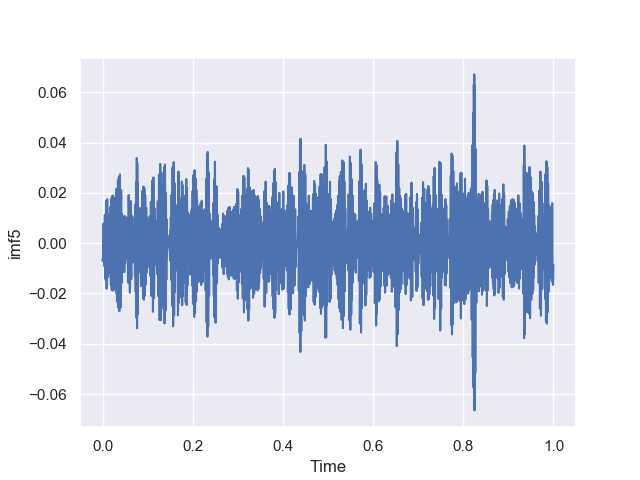
\includegraphics[width=2in]{imf/imf5.png} 
     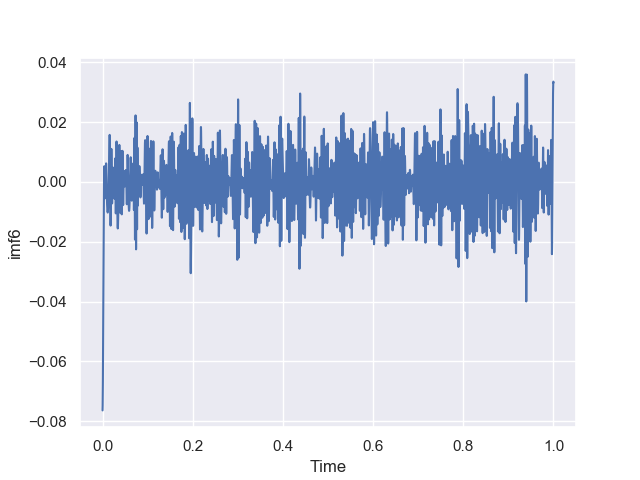
\includegraphics[width=2in]{imf/imf6.png} 
   \caption{5th and 6th intrinsic mode function (imf)}
   \label{fig:imf56}
\end{figure}

\begin{figure}[H] %  figure placement: here, top, bottom, or page
   \centering
   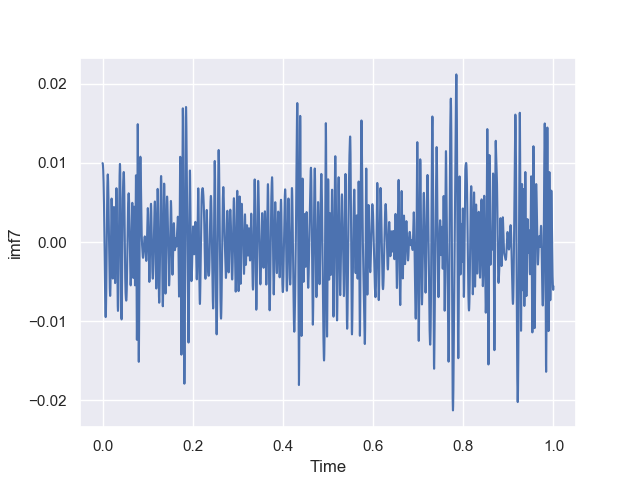
\includegraphics[width=2in]{imf/imf7.png} 
     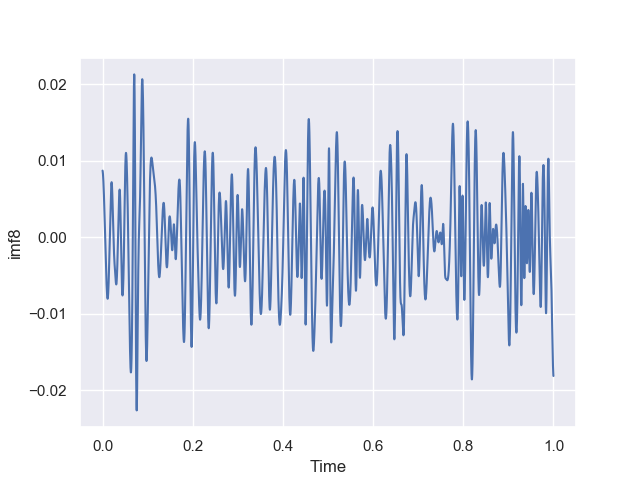
\includegraphics[width=2in]{imf/imf8.png} 
   \caption{7th and 8th intrinsic mode function (imf)}
   \label{fig:imf78}
\end{figure}

\begin{figure}[H] %  figure placement: here, top, bottom, or page
   \centering
   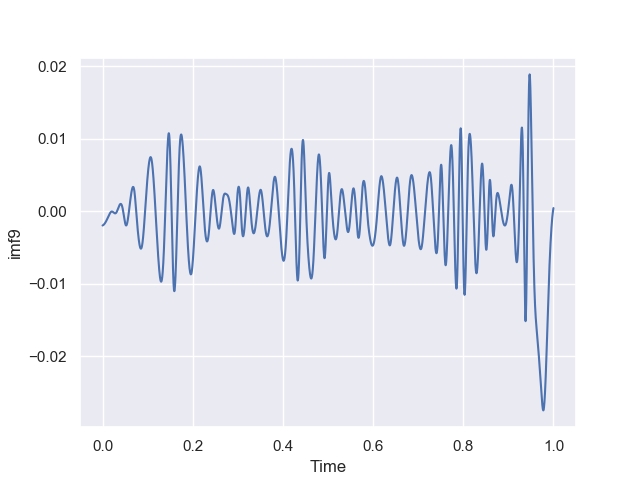
\includegraphics[width=2in]{imf/imf9.png} 
     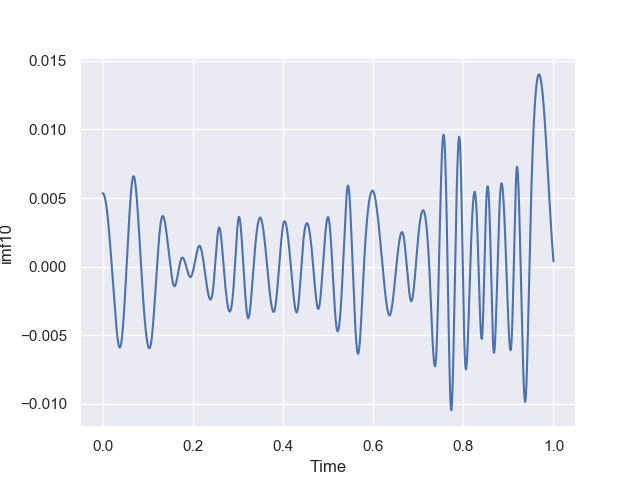
\includegraphics[width=2in]{imf/imf10.png} 
   \caption{9th and 10th intrinsic mode function (imf)}
   \label{fig:imf910}
\end{figure}

\begin{figure}[H] %  figure placement: here, top, bottom, or page
   \centering
   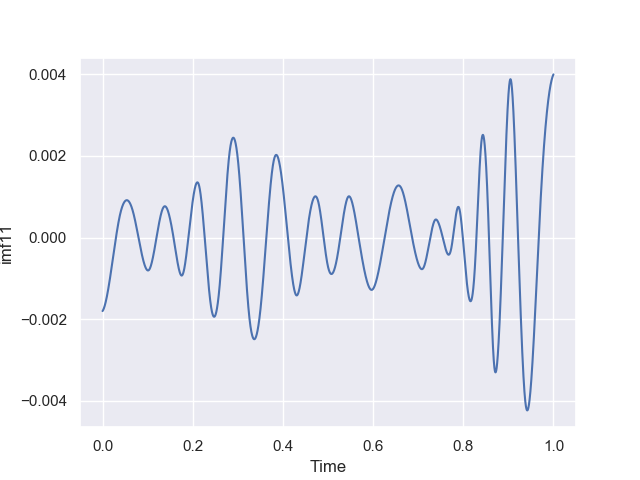
\includegraphics[width=2in]{imf/imf11.png} 
     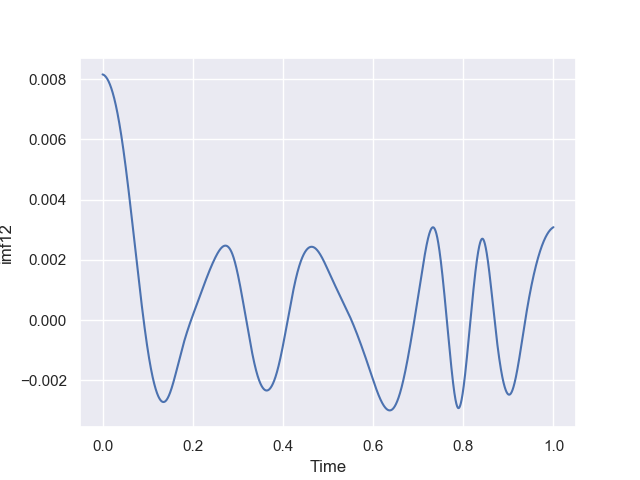
\includegraphics[width=2in]{imf/imf12.png} 
   \caption{11th and 12th intrinsic mode function (imf)}
   \label{fig:imf1112}
\end{figure}

\begin{figure}[H] %  figure placement: here, top, bottom, or page
   \centering
   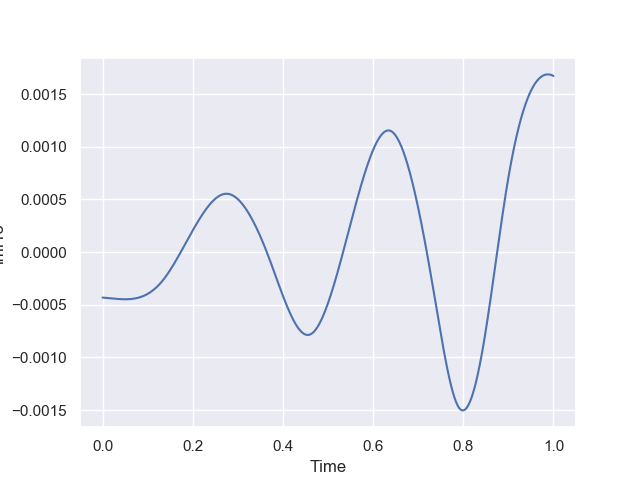
\includegraphics[width=2in]{imf/imf13.png} 
     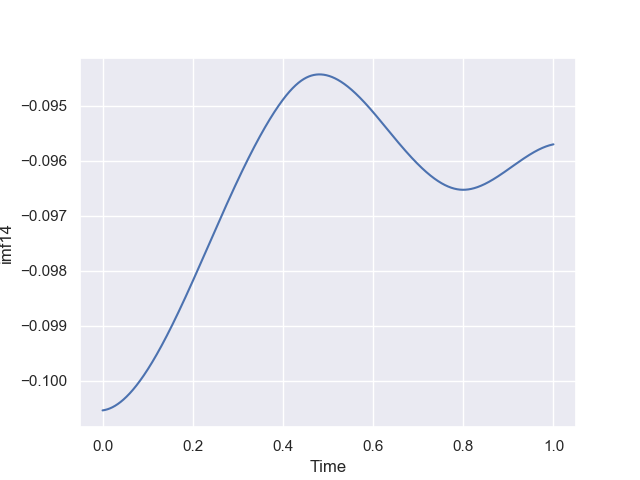
\includegraphics[width=2in]{imf/imf14.png} 
   \caption{13th and 14th intrinsic mode function (imf)}
   \label{fig:imf1314}
\end{figure}

\end{flushleft}

%\begin{figure}[H] %  figure placement: here, top, bottom, or page
%   \centering
%   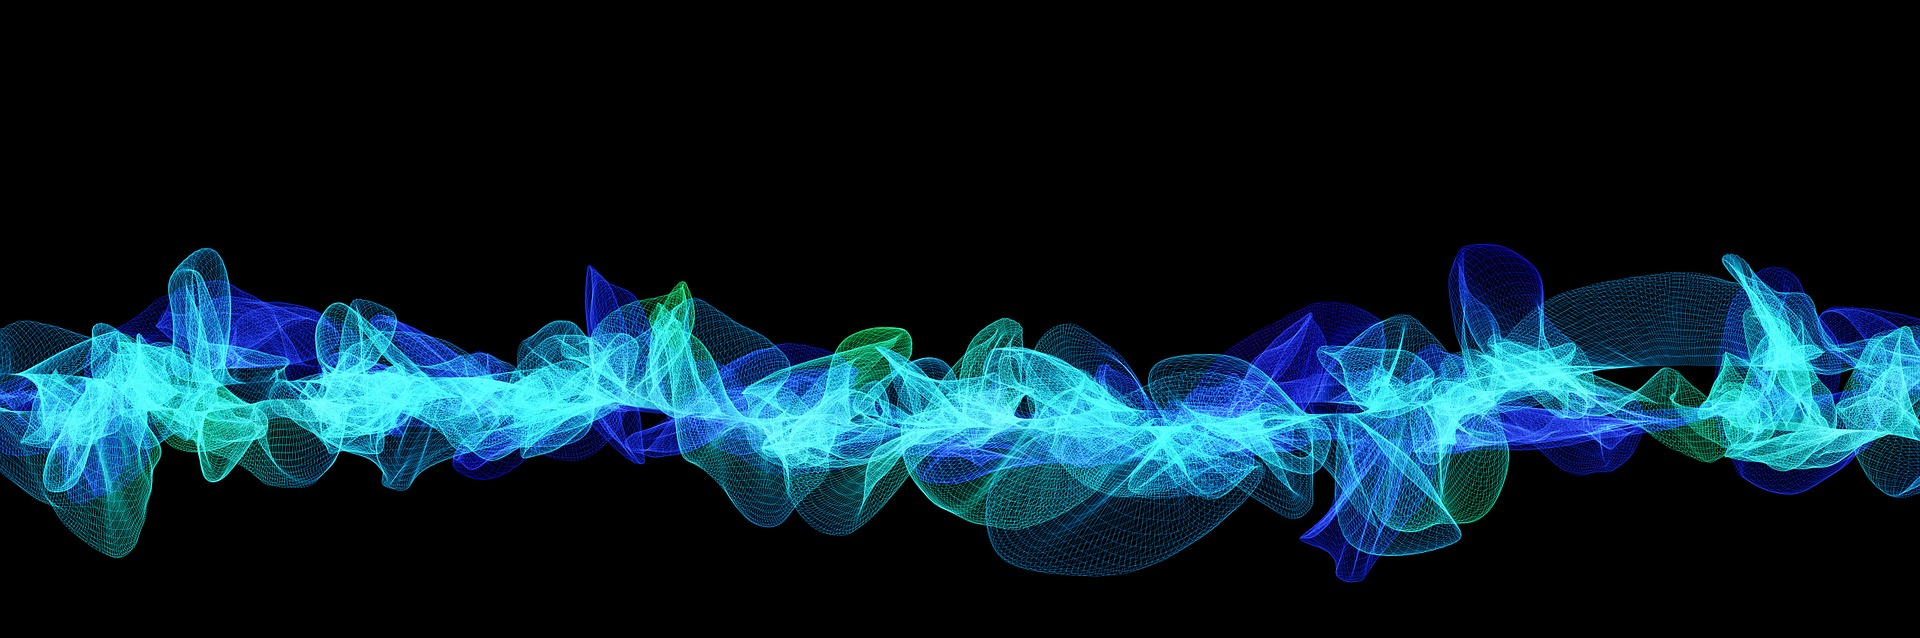
\includegraphics[width=4in]{vibration} 
%   \caption{}
%   \label{fig:example}
%\end{figure}
%In this approach we use the old goody Fourier transform. Firstly, we need the defect frequency for the outer race defect and the inner race defect. The bearing type used are Rexnor ZA-2115. For this type of bearing, the constant defect frequency (cdf) for ball pass frequency outer race defect is 0.1182 and the constant defect frequency for ball pass frequency inner race defect is 0.1484 [reference]. According to Rexnord product engineering group [reference, last page], to find the defect frequency in Hz we multiply the constant defect frequency (cdf) by the rotational speed of the bearing ( here 2000 RPM), to find the defect frequency in Hz. Note that the defect frequency is computed from the geometry of the bearing, which means that for a specific bearing, this is a constant value.
%


%\begin{flushleft}
%\begin{figure}[H] %  figure placement: here, top, bottom, or page
%   \centering
%   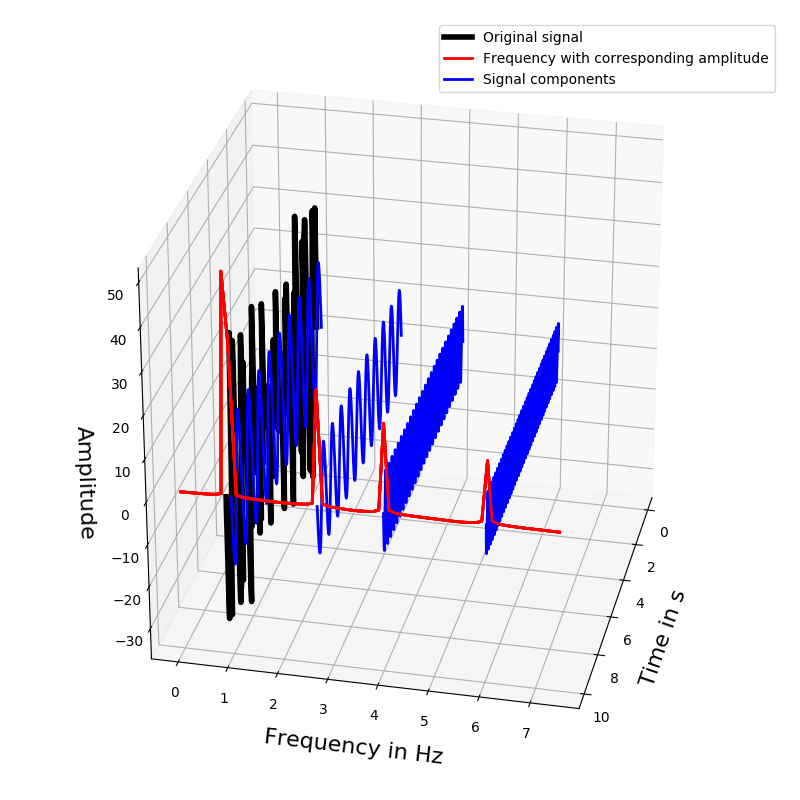
\includegraphics[width=4in]{decomposition} 
%   \caption{example caption}
%   \label{fig:example}
%\end{figure}
%
%
%
%Next, we compute the envelop spectrum for each vibration signal by using the FFT method (Fast Fourier Transform). The envelop spectrum is used to detect early sign of failure. Recall that a vibration signal can be decomposed into its sub components, where each  sub component 
%is characterised by its frequency and its amplitude. Early sign of failure can be seen in the high frequency low amplitude sub component. As the failure becomes more pronounced, it becomes visible in the low frequency high amplitude sub component.
%\end{flushleft}
%
%\begin{figure}[H] %  figure placement: here, top, bottom, or page
%   \centering
%   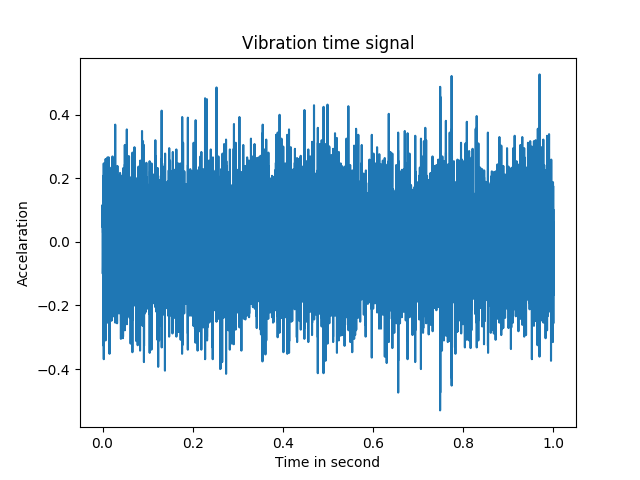
\includegraphics[width=4in]{time-signal.png} 
%   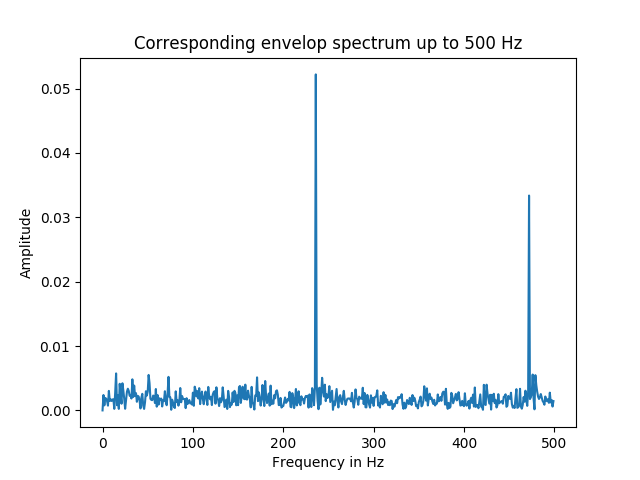
\includegraphics[width=4in]{spectrum.png} 
%      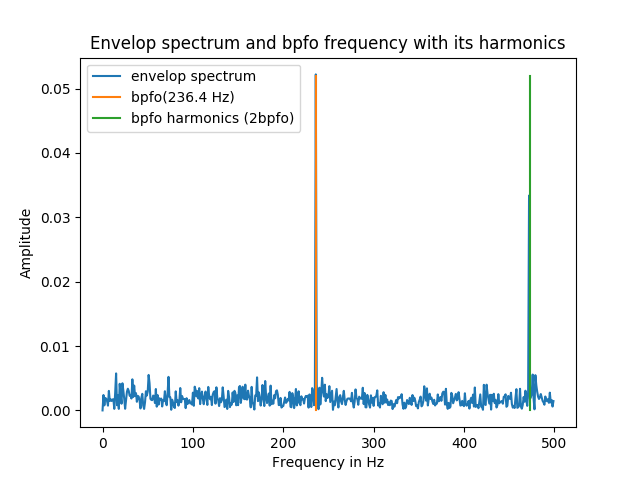
\includegraphics[width=4in]{fault.png} 
%   \caption{Vibration time signal}
%   \label{fig:signal}
%\end{figure}
%By computing the envelop spectrum for each time signal and extracting the amplitude of a defect frequency we can visualise the severity of a defect
%
%\begin{figure}[H] %  figure placement: here, top, bottom, or page
%   \centering
%   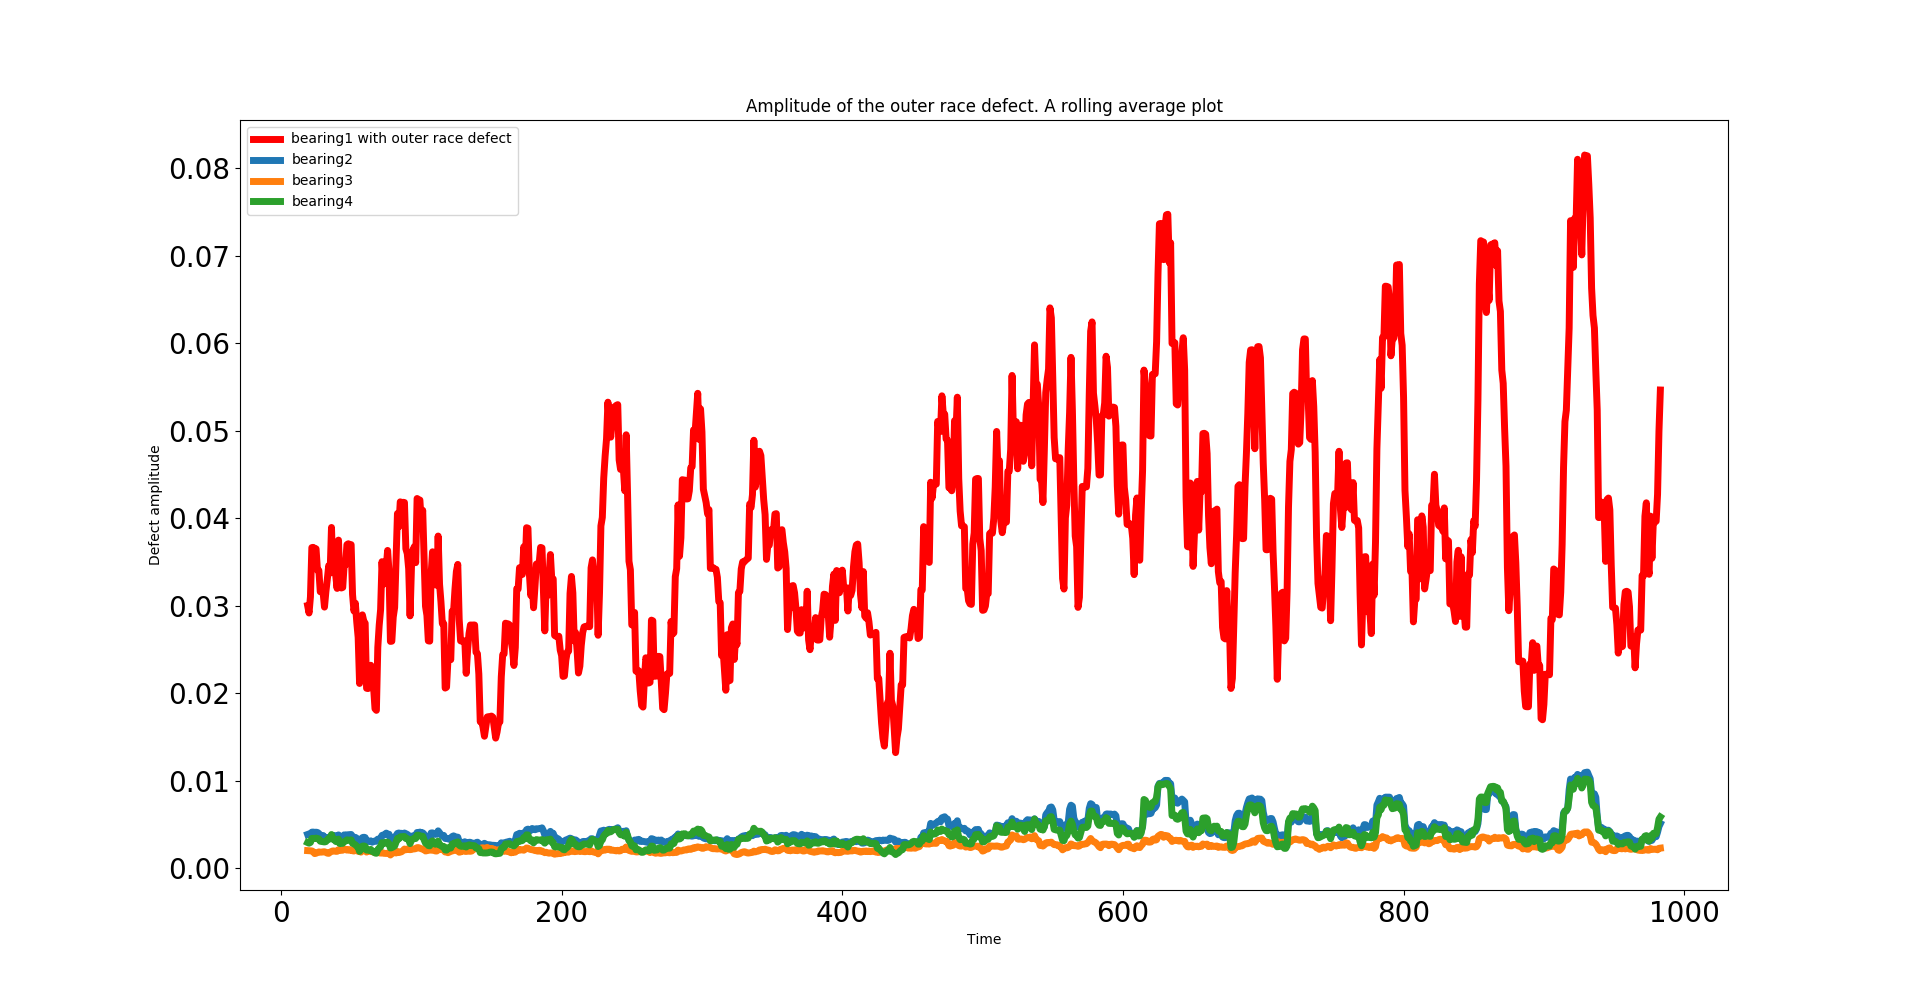
\includegraphics[width=7in]{signal_processing_method_bpfo} 
%   \caption{Ball pass frequency outer race detection}
%   \label{fig:example}
%\end{figure}
%
%\begin{figure}[H] %  figure placement: here, top, bottom, or page
%   \centering
%   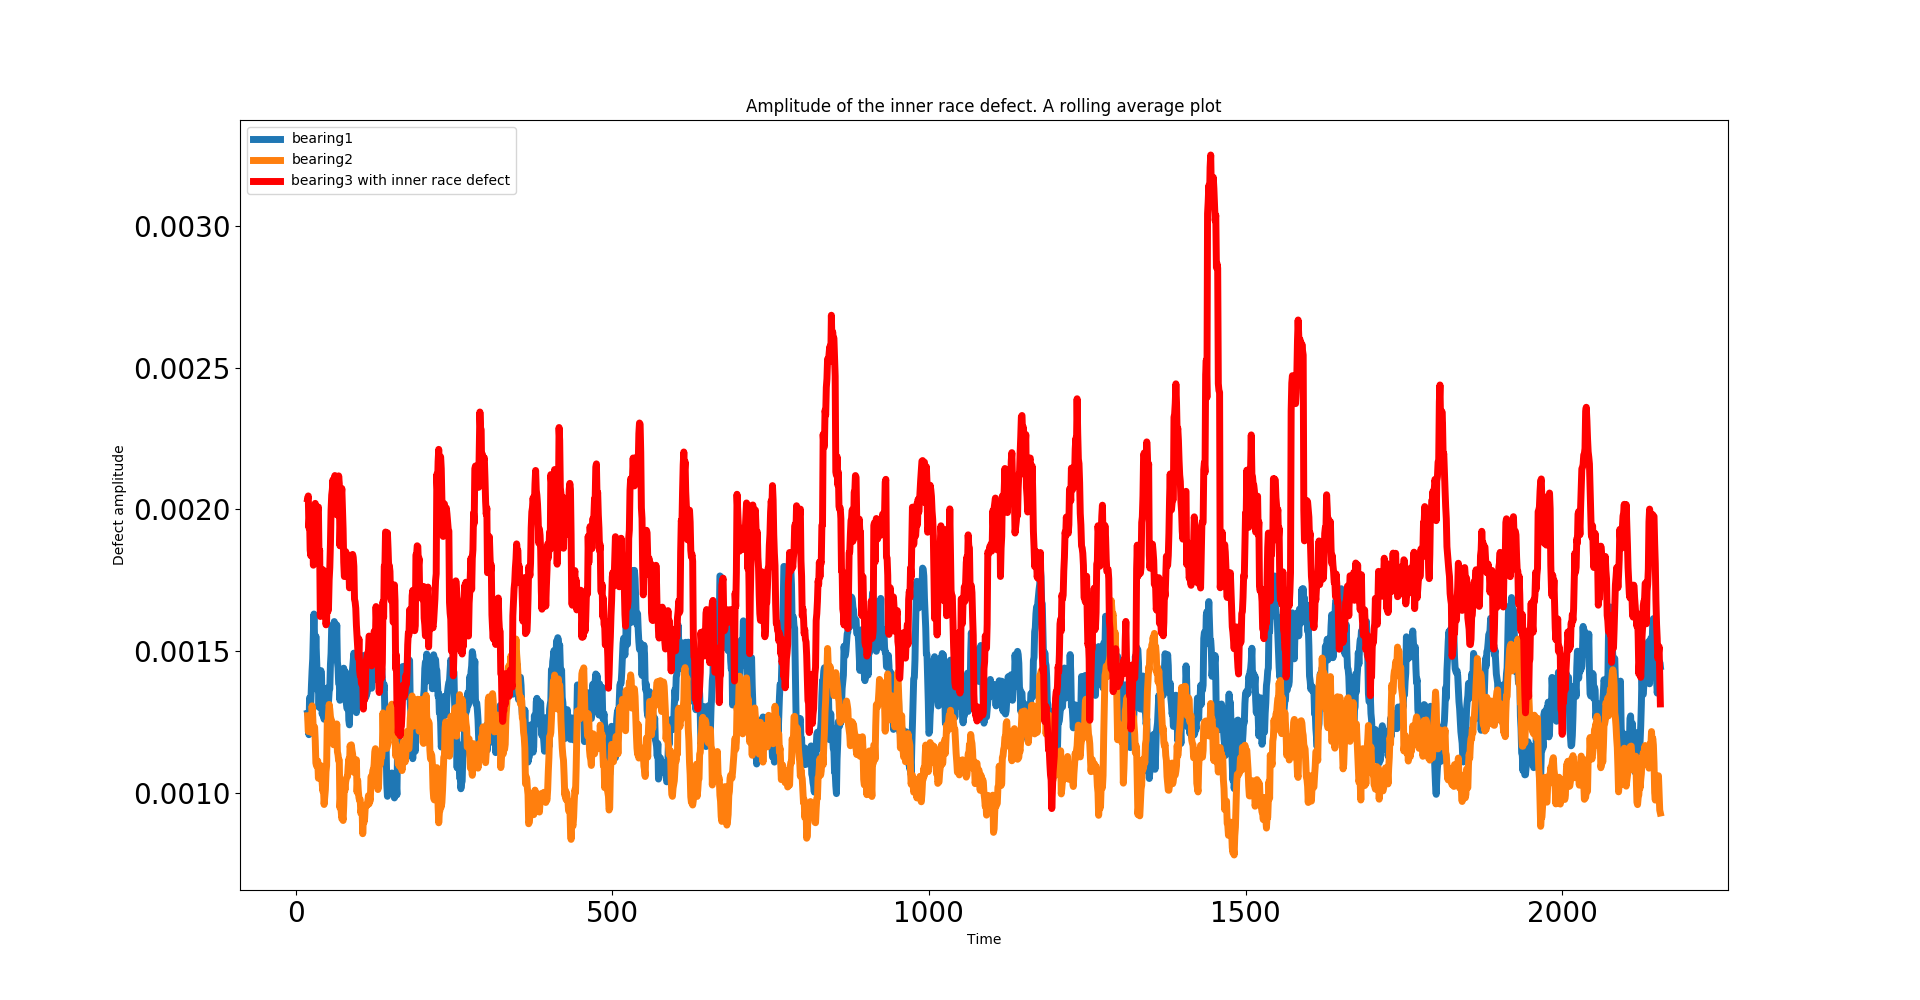
\includegraphics[width=7in]{signal_processing_method_bpfi} 
%   \caption{Ball pass frequency inner race detection}
%   \label{fig:example}
%\end{figure}
%

%%%%%%%%%%%%%%%%%%%%%%%%%%%%%%%%%%%%%%%%%%%%%%%%%%%%%%%%%%%%%%%%%%%%%%%%%%%%%%%%%%%%
%%%%%%%%%%%%%%%%%%%%%%%%%%%%%%%%%%%%%%%%%%%%%%%%%%%%%%%%%%%%%%%%%%%%%%%%%%%%%%%%%%%%
%%%%%%%%%%%%%%%%%%%%%%%%%%%%%%%%%%%%%%%%%%%%%%%%%%%%%%%%%%%%%%%%%%%%%%%%%%%%%%%%%%%%
\section{Machine learning methods}
\subsection{Overview}




\section{Result}
\subsection{Overview}
We apply the methodology described in this work to an application for bearing fault detection.
\begin{figure}[H] %  figure placement: here, top, bottom, or page
   \centering
   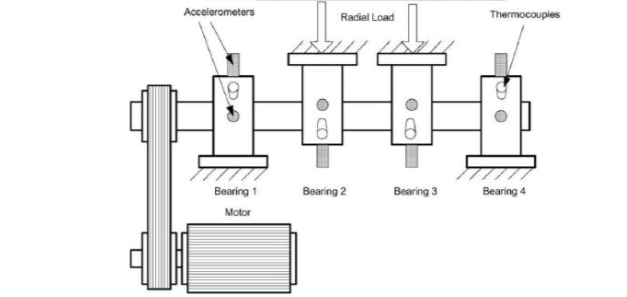
\includegraphics[width=4in]{experiment} 
   \caption{Experimental set up}
   \label{fig:exp}
\end{figure}
The data used in this use case was generated by the Intelligence Maintenance system (IMS) [link to the IMS].
Three separate experiments involving four bearings were performed on a motor. In each experiment, a 1-second vibration signal snapshots was recorded every 10 minutes, for a specified time. Each vibrational signal sample consists of 20 480 data points with sampling rate of 20 000 Hz.
In this post I will be using the first and the second experiment data [available here (give a link to the data)].


\section{Conclusion}
\begin{thebibliography}{9}
\bibitem{norden2008} 
Norden E. Huang and Zhaohua Wu 
\textit{A review on Hilbert-Huang Transform: Methods and its Application to Geophysical Studies}. 
Review of Geophysics, 2008
 
\bibitem{norden1998} 
Norden E. Huang, Zheng Shen, Steven R. Long, Manlic C. Wu, Hsing H.Shih, Quanan Zheng, Nai-Chyuan Yen, Chi Chao Tung and Henry H. Liu
\textit{The Empirical mode decomposition and the Hilbert Spectrum for nonlinear and non-stationary time series analysis}
Proc. R. Soc. Lond. A (1998) 455, 903:?995.
 
\bibitem{hui2007} 
Hui Li, Yuping Zhang and Haiqi Zheng
\textit{Hilbert-Huang transform and marginal spectrum for detecting and diagnosis of localized defects in roller bearings}
Journal of Mechanical Technology, 2007
\end{thebibliography}






\end{document}  